%%%%%%%%%%%%%%%%%%%%%%%%%%%%%%%%%%%%%%%%%
% Masters/Doctoral Thesis 
% LaTeX Template
% Version 2.5 (27/8/17)
%
% This template was downloaded from:
% http://www.LaTeXTemplates.com
%
% Version 2.x major modifications by:
% Vel (vel@latextemplates.com)
%
% This template is based on a template by:
% Steve Gunn (http://users.ecs.soton.ac.uk/srg/softwaretools/document/templates/)
% Sunil Patel (http://www.sunilpatel.co.uk/thesis-template/)
%
% Template license:
% CC BY-NC-SA 3.0 (http://creativecommons.org/licenses/by-nc-sa/3.0/)
%
%%%%%%%%%%%%%%%%%%%%%%%%%%%%%%%%%%%%%%%%%

%----------------------------------------------------------------------------------------
%	PACKAGES AND OTHER DOCUMENT CONFIGURATIONS
%----------------------------------------------------------------------------------------

\documentclass[
11pt, % The default document font size, options: 10pt, 11pt, 12pt
oneside, % Two side (alternating margins) for binding by default, uncomment to switch to one side
english, % ngerman for German
singlespacing, % Single line spacing, alternatives: onehalfspacing or doublespacing
%draft, % Uncomment to enable draft mode (no pictures, no links, overfull hboxes indicated)
%nolistspacing, % If the document is onehalfspacing or doublespacing, uncomment this to set spacing in lists to single
%liststotoc, % Uncomment to add the list of figures/tables/etc to the table of contents
%toctotoc, % Uncomment to add the main table of contents to the table of contents
%parskip, % Uncomment to add space between paragraphs
%nohyperref, % Uncomment to not load the hyperref package
headsepline, % Uncomment to get a line under the header
%chapterinoneline, % Uncomment to place the chapter title next to the number on one line
%consistentlayout, % Uncomment to change the layout of the declaration, abstract and acknowledgements pages to match the default layout
]{MastersDoctoralThesis} % The class file specifying the document structure

\usepackage{fourier} % Use the Palatino font by default
\usepackage[T1]{fontenc} % Output font encoding for international characters
\usepackage[utf8]{inputenc} % Required for inputting international characters
\usepackage{siunitx}
\usepackage{mathtools}
\usepackage{subfig}
\usepackage{caption}
\usepackage[inline]{enumitem}
\usepackage[final]{microtype}
\usepackage[backend=bibtex,style=alphabetic,natbib=true]{biblatex} % Use the bibtex backend with the authoryear citation style (which resembles APA)

\addbibresource{tesis.bib} % The filename of the bibliography

\usepackage[autostyle=true]{csquotes} % Required to generate language-dependent quotes in the bibliography

%----------------------------------------------------------------------------------------
%	MARGIN SETTINGS
%----------------------------------------------------------------------------------------

\geometry{
	paper=letterpaper, % Change to letterpaper for US letter
	inner=2.5cm, % Inner margin
	outer=3.5cm, % Outer margin
	bindingoffset=.5cm, % Binding offset
	top=1.5cm, % Top margin
	bottom=1.5cm, % Bottom margin
	% showframe, % Uncomment to show how the type block is set on the page
}

%----------------------------------------------------------------------------------------
%	THESIS INFORMATION
%----------------------------------------------------------------------------------------

\thesistitle{Thesis Title} % Your thesis title, this is used in the title and abstract, print it elsewhere with \ttitle
\supervisor{Dr. James \textsc{Smith}} % Your supervisor's name, this is used in the title page, print it elsewhere with \supname
\examiner{} % Your examiner's name, this is not currently used anywhere in the template, print it elsewhere with \examname
\degree{Doctor of Philosophy} % Your degree name, this is used in the title page and abstract, print it elsewhere with \degreename
\author{John \textsc{Smith}} % Your name, this is used in the title page and abstract, print it elsewhere with \authorname
\addresses{} % Your address, this is not currently used anywhere in the template, print it elsewhere with \addressname

\subject{Biological Sciences} % Your subject area, this is not currently used anywhere in the template, print it elsewhere with \subjectname
\keywords{} % Keywords for your thesis, this is not currently used anywhere in the template, print it elsewhere with \keywordnames
\university{\href{http://www.university.com}{University Name}} % Your university's name and URL, this is used in the title page and abstract, print it elsewhere with \univname
\department{\href{http://department.university.com}{Department or School Name}} % Your department's name and URL, this is used in the title page and abstract, print it elsewhere with \deptname
\group{\href{http://researchgroup.university.com}{Research Group Name}} % Your research group's name and URL, this is used in the title page, print it elsewhere with \groupname
\faculty{\href{http://faculty.university.com}{Faculty Name}} % Your faculty's name and URL, this is used in the title page and abstract, print it elsewhere with \facname

\AtBeginDocument{
\hypersetup{pdftitle=\ttitle} % Set the PDF's title to your title
\hypersetup{pdfauthor=\authorname} % Set the PDF's author to your name
\hypersetup{pdfkeywords=\keywordnames} % Set the PDF's keywords to your keywords
}

\begin{document}

\frontmatter % Use roman page numbering style (i, ii, iii, iv...) for the pre-content pages

\pagestyle{plain} % Default to the plain heading style until the thesis style is called for the body content

%----------------------------------------------------------------------------------------
%	TITLE PAGE
%----------------------------------------------------------------------------------------

\begin{titlepage}
\begin{center}

\vspace*{.06\textheight}
{\scshape\LARGE \univname\par}\vspace{1.5cm} % University name
\textsc{\Large Doctoral Thesis}\\[0.5cm] % Thesis type

\HRule \\[0.4cm] % Horizontal line
{\huge \bfseries \ttitle\par}\vspace{0.4cm} % Thesis title
\HRule \\[1.5cm] % Horizontal line
 
\begin{minipage}[t]{0.4\textwidth}
\begin{flushleft} \large
\emph{Author:}\\
\href{http://www.johnsmith.com}{\authorname} % Author name - remove the \href bracket to remove the link
\end{flushleft}
\end{minipage}
\begin{minipage}[t]{0.4\textwidth}
\begin{flushright} \large
\emph{Supervisor:} \\
\href{http://www.jamessmith.com}{\supname} % Supervisor name - remove the \href bracket to remove the link  
\end{flushright}
\end{minipage}\\[3cm]
 
\vfill

\large \textit{A thesis submitted in fulfillment of the requirements\\ for the degree of \degreename}\\[0.3cm] % University requirement text
\textit{in the}\\[0.4cm]
\groupname\\\deptname\\[2cm] % Research group name and department name
 
\vfill

{\large \today}\\[4cm] % Date
%\includegraphics{Logo} % University/department logo - uncomment to place it
 
\vfill
\end{center}
\end{titlepage}

%----------------------------------------------------------------------------------------
%	QUOTATION PAGE
%----------------------------------------------------------------------------------------

\vspace*{0.2\textheight}

\noindent\enquote{\itshape Thanks to my solid academic training, today I can write hundreds of words on virtually any topic without possessing a shred of information, which is how I got a good job in journalism.}\bigbreak

\hfill Dave Barry

%----------------------------------------------------------------------------------------
%	ABSTRACT PAGE
%----------------------------------------------------------------------------------------

\begin{abstract}
\addchaptertocentry{\abstractname} % Add the abstract to the table of contents
The Thesis Abstract is written here (and usually kept to just this page). The page is kept centered vertically so can expand into the blank space above the title too\ldots
\end{abstract}

%----------------------------------------------------------------------------------------
%	ACKNOWLEDGEMENTS
%----------------------------------------------------------------------------------------

\begin{acknowledgements}
\addchaptertocentry{\acknowledgementname} % Add the acknowledgements to the table of contents
The acknowledgments and the people to thank go here, don't forget to include your project advisor\ldots
\end{acknowledgements}

%----------------------------------------------------------------------------------------
%	LIST OF CONTENTS/FIGURES/TABLES PAGES
%----------------------------------------------------------------------------------------

\tableofcontents % Prints the main table of contents

\listoffigures % Prints the list of figures

\listoftables % Prints the list of tables

%----------------------------------------------------------------------------------------
%	ABBREVIATIONS
%----------------------------------------------------------------------------------------

% \begin{abbreviations}{ll} % Include a list of abbreviations (a table of two columns)

% \textbf{LAH} & \textbf{L}ist \textbf{A}bbreviations \textbf{H}ere\\
% \textbf{WSF} & \textbf{W}hat (it) \textbf{S}tands \textbf{F}or\\

% \end{abbreviations}

%----------------------------------------------------------------------------------------
%	PHYSICAL CONSTANTS/OTHER DEFINITIONS
%----------------------------------------------------------------------------------------

% \begin{constants}{lr@{${}={}$}l} % The list of physical constants is a three column table

% % The \SI{}{} command is provided by the siunitx package, see its documentation for instructions on how to use it

% Speed of Light & $c_{0}$ & \SI{2.99792458e8}{\meter\per\second} (exact)\\
% %Constant Name & $Symbol$ & $Constant Value$ with units\\

% \end{constants}

%----------------------------------------------------------------------------------------
%	SYMBOLS
%----------------------------------------------------------------------------------------

% \begin{symbols}{lll} % Include a list of Symbols (a three column table)

% $a$ & distance & \si{\meter} \\
% $P$ & power & \si{\watt} (\si{\joule\per\second}) \\
% %Symbol & Name & Unit \\

% \addlinespace % Gap to separate the Roman symbols from the Greek

% $\omega$ & angular frequency & \si{\radian} \\

% \end{symbols}

%----------------------------------------------------------------------------------------
%	DEDICATION
%----------------------------------------------------------------------------------------

\dedicatory{For/Dedicated to/To my\ldots} 

%----------------------------------------------------------------------------------------
%	THESIS CONTENT - CHAPTERS
%----------------------------------------------------------------------------------------

\mainmatter % Begin numeric (1,2,3...) page numbering

\pagestyle{thesis} % Return the page headers back to the "thesis" style

% Include the chapters of the thesis as separate files from the Chapters folder
% Uncomment the lines as you write the chapters

%%--------- Comandos especiales
\newcommand{\vecr}{\mathbf{r}}
\newcommand{\veck}{\mathbf{k}}
\newcommand{\nnet}{N_{\theta}(\mathbf{r})}
%%
\chapter{Neural networks as an approximation for the bridge function} % Main chapter title

\label{Cap3}

%----------------------------------------------------------------------------------------
%	SECTION 1
%----------------------------------------------------------------------------------------

Neural networks can be used as \emph{universal approximators}~\cite{hornikMultilayerFeedforwardNetworks1989, hornikApproximationCapabilitiesMultilayer1991, cybenkoApproximationSuperpositionsSigmoidal1989},
in other words, they can take the form of any continuous function for some specific
types of architectures.
In particular, it is hypothesized that a neural network might be useful as a bridge function
parametrization in the closure expression for the Ornstein-Zernike equation. If this is true,
then choosing a particular approximation can be avoided for a given interaction potential, 
and leave the choice of the bridge function to the neural network itself, while
simultaneously solving the Ornstein-Zernike equation.

In this chapter, we show in detail the methodology created to achieve such a task, and
the mathematical structure with which a neural network can be used to solve the
Ornstein-Zernike equation.
These results are compared to those obtained from computer simulations to assess the
quality of the solution.
In the appendix, the detailed algorithm used to solve the Ornstein-Zernike equation
is presented, along with a detailed computation of the gradients used for the
training scheme. Here, we shall focus only on the main results and the algorithm structure
in general.

\section{Parametrization of the bridge function}

The Ornstein-Zernike equation is given by the following expression

\begin{subequations}
    \begin{align*}
         & h(\vecr) = c(\vecr) +
        n \int_{V}
        c(\vecr^{\prime})
        h(\lvert \vecr - \vecr^{\prime} \rvert)
        d\vecr^{\prime} \label{eq:oz1} \\
         & c(\vecr)
        = \exp{\left[
                -  \beta u(\vecr)
                +  \gamma(\vecr)
                + B(\vecr)
                \right]} -
        \gamma(\vecr)
        - 1
    \end{align*}
\end{subequations}

with the already known notation for each quantity (Ref a marco teórico).

Let $\nnet$ be a neural network with weights $\theta$. The main hypothesis
of this chapter is that $\nnet$ can replace the bridge function $B(\vecr)$
in the previous equation, which will yield the following expression for
the closure relation

\begin{equation}
    c(\vecr) = \exp{\left[
            -  \beta u(\vecr)
            +  \gamma(\vecr)
            + \nnet
            \right]} -
    \gamma(\vecr)
    - 1 .
    \label{eq:parametrizacion}
\end{equation}

With this new expression, the main problem to solve is to find the weights
of $\nnet$ that can successfully solve the Ornstein-Zernike equation
for a given interaction potential, $\beta u(\vecr)$.

%----------------------------------------------------------------------------------------
%	SECTION 2
%----------------------------------------------------------------------------------------

\section{Training scheme}
Now that a parametrization is defined, a way to fit the weights of the neural network must
be devised. This new numerical scheme must also be able to solve the OZ equation, while
simultaneously finding the appropiate weights for $\nnet$.

\subsection{Cost function}
It was mentioned previously that the main problem to solve is to find the weights of
$\nnet$ that can successfully solve the Ornstein-Zernike equation
for a given interaction potential.
To solve such problem, a \textbf{cost function} must be defined, and be used as part of
a \emph{minimization} problem.

To define such a function, we consider the successive approximations obtained from the
iterative Piccard scheme to solve the OZ equation, $\{\gamma_1(\vecr), \gamma_2(\vecr), \dots, \gamma_n(\vecr)\}$.
From this, we expect to have found a solution when each approximation
is \emph{close enough} to the previous one. This can be translated into the following
cost function

\begin{equation}
    J(\theta) = \left[\gamma_{n}(\vecr; \theta) - \gamma_{n-1}(\vecr; \theta) \right]^2
    \label{eq:costo}
\end{equation}

where $\gamma_{n}(\vecr; \theta)$ is the $n$-th approximation of the indirect
correlation function, $\gamma(\vecr)$.
The notation $\gamma(\vecr; \theta)$ indicates that the function now depends implicitly
on the weights of the neural network, as seen in equation~\eqref{eq:parametrizacion}.
This means that, if the weights of $\nnet$ change, we should expect a change in the output
from the $\gamma$ function. Nevertheless, this does not mean that the indirect
correlation function itself depends explicitly, nor directly, on the weights of
$\nnet$.

Another way of looking at expression~\eqref{eq:costo} is that we require that the last 
two approximations of the $\gamma$ function in each iteration from the numerical scheme to 
be as equal as possible. This will enforce a change on the weights every time both 
approximations deviate between them.

\subsection{Optimization problem}
With a cost function at hand, an optimization problem can be defined such that the
weights of $\nnet$ will be adjusted properly.

This optimization problem is in fact an \emph{unconstrained optimization problem},
and it is defined simply as

\begin{equation}
    \begin{aligned}
         & \underset{\theta}{\text{min}}
         & & J(\theta)
    \end{aligned}
    .
    \label{eq:optimizacion}
\end{equation}

This formulation is just a search for the best values for the weights that minimize
the squared difference between successive approximations.
This optimization problem can be solved iteratively, along with the solution of the
OZ equation, which is also an iterative process.

\subsection{Weight updates}
The iterative method employed to adjust the weights of $\nnet$ is based on the
\emph{gradient descent} method~\cite{nocedalNumericalOptimization2006}.
The most general update rule for a method based on gradient descent reads

\begin{equation}
    \theta_{n+1} = \theta_n - \eta \nabla_{\theta} J(\theta) .
    \label{eq:gradiente}
\end{equation}

where $\eta$ is known as the \emph{learning rate}, and it is a hyperparameter
that controls the step size at each iteration while moving toward the minimum
of a cost function. This value needs to be \emph{tuned} accordingly, so
that the method converges properly.

Regardless of the particular expression for the weight updates, every method
based on the gradient descent method \emph{requires} the gradient information from
the cost function with respect to the weights, $\nabla_{\theta} J(\theta)$.
In this particular case, the detailed computation of the gradient is described in
the appendix~\ref{AppendixA}.
Once this information is obtained, all that is left is to build an algorithm that
can correctly use this training scheme and solve the OZ equation.

\subsection{Solving the Ornstein-Zernike equation with neural networks}
Having described all the necessary elements needed, a general layout for the solution
of the Ornstein-Zernike using neural networks is now presented.

Thus, we propose the following steps to solve the OZ using the parametrization~\eqref{eq:parametrizacion}:

\begin{enumerate}
    \item Given a particular interaction potential $\beta u(\vecr)$, equation~\eqref{eq:parametrizacion} is used to obtain the value of the direct correlation function $c(\vecr; \theta)$, which now depends implicitly on the weights of $\nnet$. In this step, an initial value for $\gamma_{n}(\vecr)$ is needed, which is initialized based on the five-point Ng methodology~\ref{AppendixA}.
    \item The newly found function $c(\vecr; \theta)$ is transformed to a reciprocal space by means of the Fourier transform yielding the new function $\hat{c}(\veck; \theta)$.
    \item Then, the full OZ equation(Ref a ec) is Fourier transformed. Using the information from the previous step, a new estimation of the indirect correlation function is obtained, $\hat{\gamma}_{n+1}(\veck; \theta)$.
    \item The Fourier transform is applied once again to return all the functions to real space. With this operation, a new estimation $\gamma_{n+1}(\vecr; \theta)$ is computed from the transformed function, $\hat{\gamma}_{n+1}(\veck; \theta)$.
    \item Both estimations, $\gamma_{n}$ and $\gamma_{n+1}$, are used to evaluate the cost function~\eqref{eq:costo}, while simultaneously computing the gradient $\nabla_{\theta} J(\theta)$.
    \item The weights $\theta$ are updated a gradient descent rule, similar to~\eqref{eq:gradiente}, and the process is repeated from step 1. In the next iteration, the initial value for the indirect correlation function will be $\gamma_{n+1}$, and a new estimation $\gamma_{n+2}$ will be obtained. This process is repeated until convergence.
\end{enumerate}

\subsection{Convergence criterion}
The procedure describe in the previous section is repeated indefinetely until convergence
is achieved. This convergence criterion is defined as follows

\begin{equation}
    \sum_{i=1}^{N} {\left( \gamma^{n+1}_{i} - \gamma^{n}_{i} \right)}^2 \leq \epsilon .
    \label{eq:tolerancia}
\end{equation}

This expression is also known as the \emph{mean squared error}~\cite{goodfellowDeepLearning2016}.
Here, we sum all the $N$ elements of the squared difference between estimates $\gamma_{n+1}$
and $\gamma_{n}$. The paramater $\epsilon \in [0,1]$ is a tolerance value that indicates an 
upper bound for the error between estimations. When the computed error is below this 
tolerance value, we consider the algorithm to have converged to a particular minimum.
Specifically, the numerical tolerance in all the experiments was fixed to be
$\epsilon = \num{1e-5}$.
This means that the weights are adjusted until the successive estimations of the $\gamma$
functions are equal between them, up to the defined tolerance $\epsilon$.

%----------------------------------------------------------------------------------------
%	SECTION 3
%----------------------------------------------------------------------------------------
\section{Implementation}
In this section we detail the most important aspects about the implementation of the
method described in the previous section. This includes the topology of the neural network,
the optimization method, and the choice of activation function. The physical parameters
as well as the computer simulations methods used to solve the OZ equation are also outlined.

\subsection{Choice of optimization algorithm}
The general rule for the weight update based on gradient descent~\eqref{eq:gradiente} was
implemented to solve the optimization problem, but numerical inconsistencies rendered this 
method unstable and convergence was almost never achieved.

To solve this issue, the \emph{Adam}~\cite{kingmaAdamMethodStochastic2017} optimization 
method was chosen. This optimization method is an excellent choice for the training
of neural networks, even more so when the gradient is expected to be \emph{sparse}, i.e.
most of the elements of the gradient itself are zeros.
The \emph{Adam} method uses several rules to adjust the descent direction of the gradient,
as well as the hyperparameters related to the acceleration mechanism of the method.
Notably, there are two important hyperparameters used by the method; $\beta_1$,
which controls the moving average of the computed gradient; and $\beta_2$, which controls
the value of the gradient squared. Both parameters are necessary for the optimal 
convergence of the algorithm.

The equations that define the optimization method are the following

\begin{align}
    m &= \beta_1 m - (1 - \beta_1) \nabla_{\theta} J(\theta) \nonumber \\
    s &= \beta_2 s + (1 - \beta_2) \nabla_{\theta} J(\theta) \odot \nabla_{\theta} J(\theta) \nonumber \\
    \hat{m} &= \frac{m}{1 - \beta_1^t} \nonumber \\
    \hat{s} &= \frac{s}{1 - \beta_2^t} \nonumber \\
    \theta &= \theta + \eta \hat{m} \oslash \sqrt{\hat{s} + \varepsilon}
    \label{eq:adam}
\end{align}

where $\odot$ is the elementwise multiplication, or Hadamard product; $\oslash$
is the elementwise division, or Hadamard division; and $\varepsilon$ is a smoothing
value to prevent division by zero.

In the results presented in this chapter, the parameters were fixed to the ones reported
as optimal in the original work~\cite{kingmaAdamMethodStochastic2017}, which are
$\beta_1=\num{0.9}$ and $\beta_2=\num{0.999}$. It is important to note that this method
has its own mechanisms to control and modify the gradients, as well as the hyperparameters.
This makes it a \emph{hands-off} method, without the need to tune the hyperparameters.
The \emph{learning rate}, $\eta$ in equation~\eqref{eq:gradiente}, was fixed to
$\eta=\num{1e-4}$ for all the experiments.

\subsection{Neural network architecture}

\begin{figure}[t]
    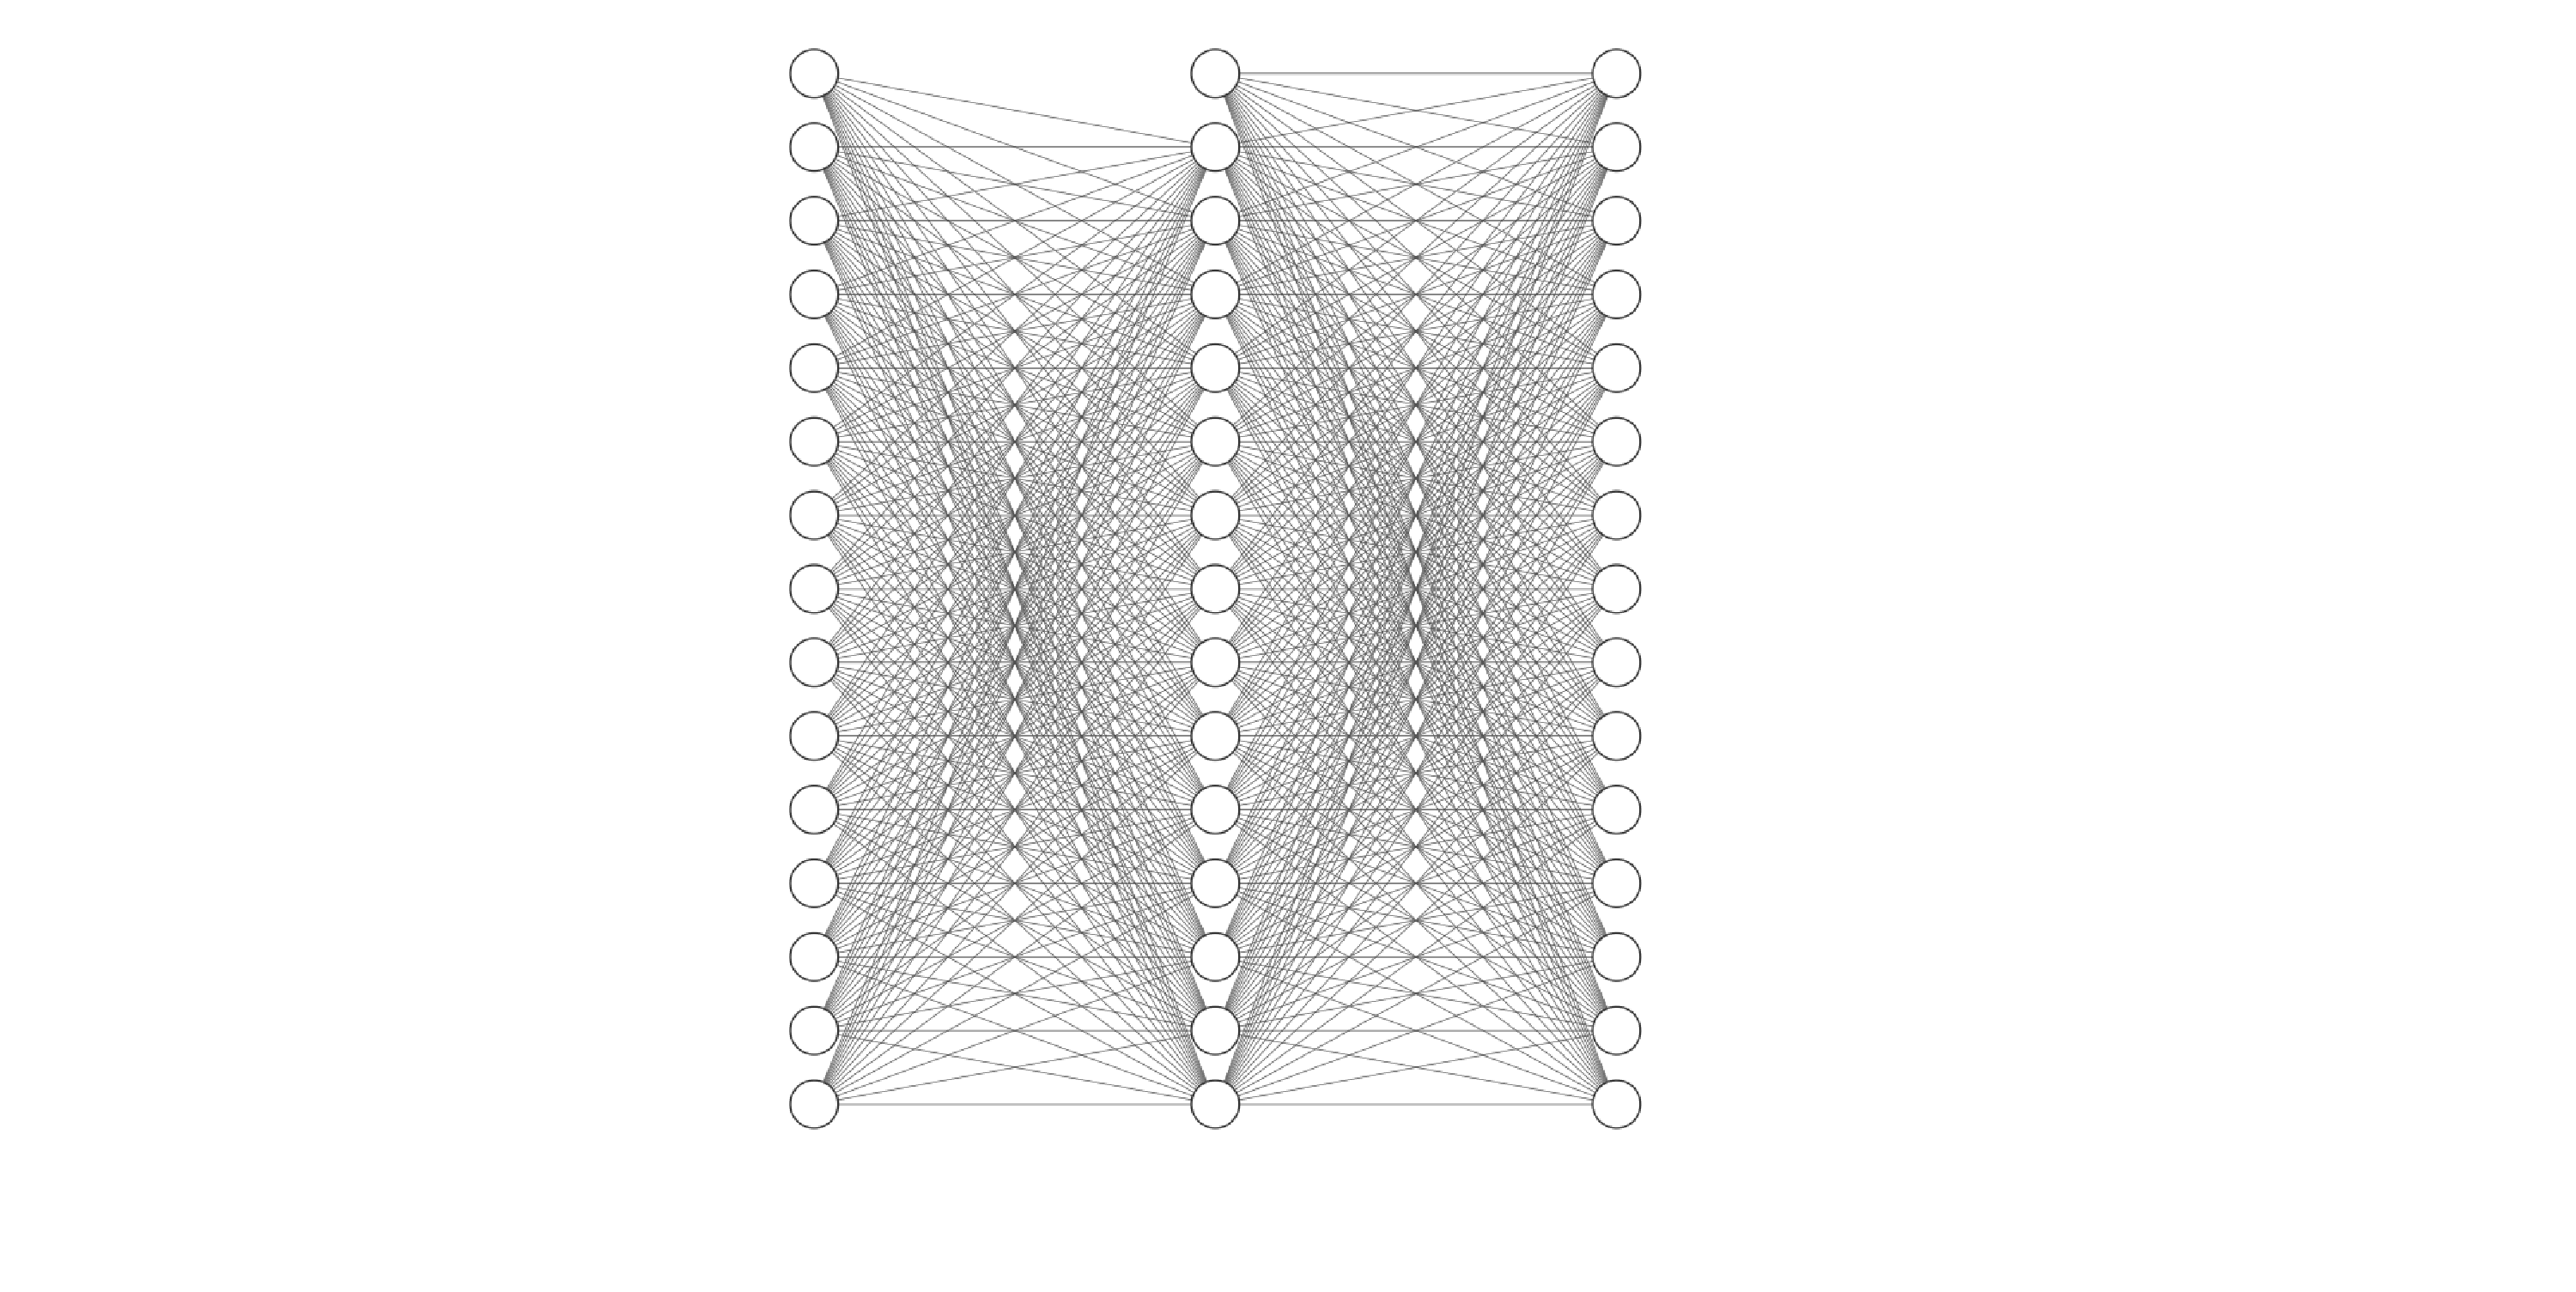
\includegraphics[width=\textwidth]{figuras/capitulo-3/neural-network.pdf}
    \vspace{-1.5cm}
    \caption[General schematics of a neural network.]{Cartoon of a fully connected multilayer neural network. Note that there is one \emph{hidden layer}. The circles represent the \emph{nodes} or \emph{units} used to compute the final output. These nodes are being evaluated by an activation function to account for nonlinearities. The top-most nodes that seem different from the main nodes are known as the \emph{bias} nodes. The real architecture used in this chapter is larger, with many more nodes and connections, but the topology is the same.}
    \label{fig:nn-esquema}
\end{figure}

The neural network architecture used in all the experiments is very similar to the one
shown in figure~\ref{fig:nn-esquema}, with the exception of the number of nodes in all the
layers.
Particularly, the neural network is made of \emph{three layers}, all connected among them.
There is an \emph{input} layer, one \emph{hidden} layer, and a final \emph{output} layer.
All layers have the same number of nodes, which is 4096. Additional nodes are added to the
final two layers that serve as the \emph{bias}.

All the weights must be initialized appropiately, and in this case the Glorot uniform
distribution was used~\cite{glorotUnderstandingDifficultyTraining2010}, which has proven
to be an excellent way to help the convergence of neural networks.
When using the Glorot uniform distribution, the weights are initialized as
$
\theta_{ij} \sim \mathcal{U} \left[ -\frac{6}{\sqrt{(in + out)}},
\frac{6}{\sqrt{(in + out)}} \right]
$,
where $\mathcal{U}$ is the uniform probability distribution;
$in$ represents the number of units in the input layer; and $out$ the number of
units in the output layer. All bias nodes were initialized to be zero.

The activation function used was the \emph{ReLU}~\cite{glorotDeepSparseRectifier2011}
function which has the form

\begin{equation*}
    \text{ReLU}(x) = \max{(0, x)} .
\end{equation*}

This activation function is applied to all the nodes in the layers, with the exception
of the input layer. This function was chosen due to the fact that the other most common
functions ($\tanh, \text{softmax}$, etc.) were numerically unstable in the training process 
of the neural network.

\subsection{Physical parameters and simulations}

To solve the OZ equation a cutoff radius of $r_c=7\sigma$ was used, where $\sigma$ is the
particle diameter and it was fixed to be $\sigma=1$.
The interaction potential used was the pseudo hard sphere potential (Ref a ec.), both
for the solution of the OZ equation as well as the results obtained from computer simulations.

Seven different densities were explored in the range $\phi \in [\num{0.15}, \num{0.45}]$, 
with $\Delta \phi = \num{0.05}$.
For each density value, a grid of 70 points was used to ensure convergence of the iterative
algorithm when solving for the OZ equation. This was not the case for the computer 
simulations, where such partition is not needed.

Computer simulations results were obtained using the traditional Monte Carlo simulation
method for the NVT ensemble (Ref a marco teórico). The total number of particles was 2197,
the system was equilibrated for a total of 10 million Monte Carlo steps, and the radial
distribution functions were obtained from the sampling of 7 million steps, after
the system was equilibrated. To reduce the number of computations, a cutoff radius of
half the size of the simulation box was used for the evaluation of the interaction 
potential. Periodic boundary conditions were applied accordingly. The same pseudo hard 
sphere potential (Ref a ecuación) was used, instead of the true hard sphere potential, for 
a fair comparison with the results obtained from the OZ equation.

%----------------------------------------------------------------------------------------
%	SECTION 4
%----------------------------------------------------------------------------------------
\section{Results}
It is now time to investigate the results obtained from the proposed methodology, using all the elements previously described.
The main point of discussion will be the radial distribution
function \textemdash $g(r^*)$ \textemdash for different values of densities, both in the
low and high density regimes.

\subsection{Low densities}
In this section we will deal with the low 
density values of $\phi=\numlist[list-pair-separator={\enspace\text{and}\enspace}]{0.15;0.25}$, which are shown in figures~(\ref{fig:rdf15}, \ref{fig:rdf25}).
The results show that, at low densities, the HNC and neural network approximations are
more precise than the modified Verlet approximation. Although, all
approximations seem to fall short compared to computer simulations. This is seen espcially
in the neighborhood around the second peak, which are represented in the insets from
figures~(\ref{fig:rdf15}, \ref{fig:rdf25}).
It is specially important to note that the neural network approximation is a little bit 
more precise than the HNC approximation, which can be qualitatively appraised by observing 
the estimation of the main peak in the radial distribution function. This peak can be found 
in the vicinity of $r^* = 1$. Nevertheless, it is still overestimated, which is the 
same case for the HNC approximation. However, this is not the case for the modified Verlet 
approximation, which undervalue the main peak.

It is also important to notice the functional form of $g(r^*)$. For the HNC and neural
network approximations, it appears to have the same form between approximations, and it 
might as well be the same. This would imply that, somehow, the weights of the neural network
were updated enough such that a minimum was found, and this minimum was very close to the
HNC approximation. In other words, the results suggest that the weights are very close to
zero, such that when the neural network is evaluated, the output is close to the
result obtained from the HNC approximation.
Another important aspect to observe is that this functional form is slightly different
to the one seen from computer simulations, and that the modified Verlet approximation is 
closer to the form found in the computer simulations results.

\subsection{High densities}
We now turn our attention to the high density values of
$\phi=\numlist[list-pair-separator={\enspace\text{and}\enspace}]{0.35; 0.45}$,
represented in figures~(\ref{fig:rdf35}, \ref{fig:rdf45}).
In the same spirit as before with the low densities, the HNC and neural network 
approximations are not precise when compared to computer simulations. In this case,
the modified Verlet bridge function approximation is even more precise, which was expected.
This is because the HNC approximation is a very good approximation for long range
interaction potentials (Ref faltante), whereas the modified Verlet is better suited for 
short range potentials, such as the one studied here.
In this case, modified Verlet is the most precise of the approximations used, which
can be appraised in figures~(\ref{fig:rdf35}, \ref{fig:rdf45}), where the 
main peak is well estimated by the approximation when compared to the computer simulation
results. However, the HNC and neural network approximation overestimate this property.

Further, the functional form of $g(r^*)$ computed with the neural network approximation 
is quite different to the one obtained with computer simulations. Indeed, the result
obtained is similar to the one obtained with the HNC approximation. This was also the
case for low densities. This result is important, backing the hypothesis that the
neural network might reduce to the HNC approximation.
This would imply that the neural network is in fact approximating the bridge function
$B(\vecr) \approx 0$. If we now pay attention to the modified Verlet
approximation, we can see that the modified Verlet bridge function is the most precise
out of all the set of bridge functions used. In other words, we observe that this
estimation predicts the main peak well, as can be seen when compared to the results
obtained from computer simulations.

\begin{figure}
    \centering
    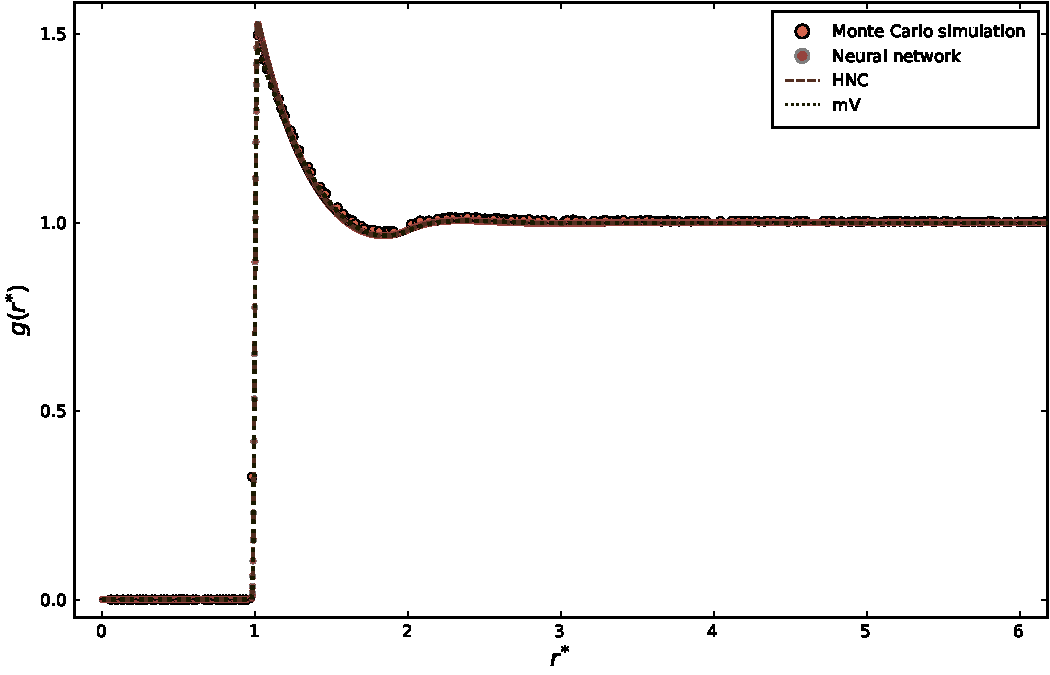
\includegraphics[width=\textwidth]{figuras/capitulo-3/comparison_p=0.15.pdf}
    \caption[Radial distribution function, $\phi=0.15$.]{The radial distribution function for density value $\phi=0.15$ obtained from computer simulations, and three different approximations:
    \begin{enumerate*}[label=(\alph*),itemjoin={,\enspace}]
        \item \emph{mV}, modified Verlet
        \item \emph{HNC}, Hypernetted Chain
        \item \emph{Neural network}, neural network approximation.
    \end{enumerate*}
    Inset shows the region close to the peak about $r^{*}=2$.
    }
    \label{fig:rdf15}
\end{figure}

\begin{figure}
    \centering
    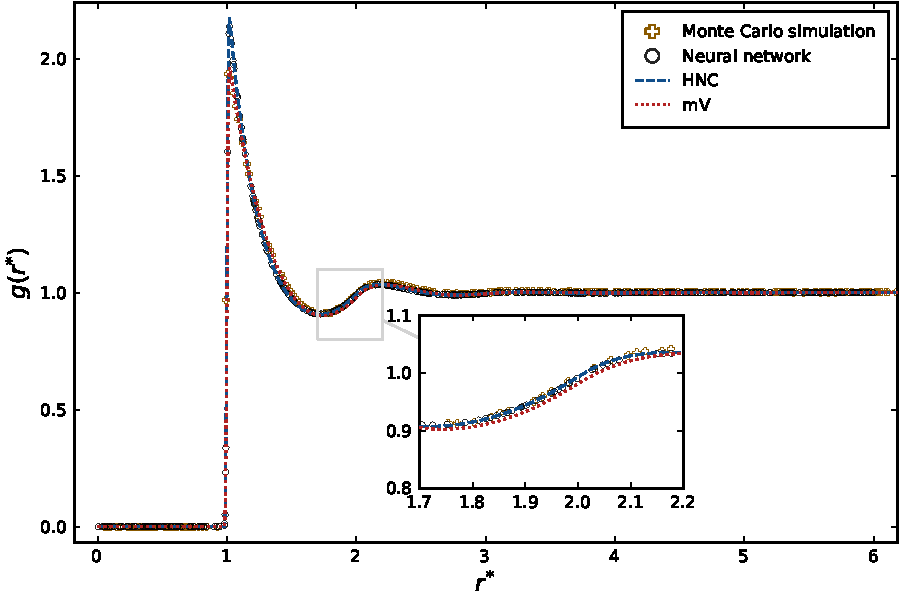
\includegraphics[width=\textwidth]{figuras/capitulo-3/comparison_p=0.25.pdf}
    \caption[Radial distribution function, $\phi=0.25$.]{The radial distribution function for density value $\phi=0.25$ obtained from computer simulations, and three different approximations:
    \begin{enumerate*}[label=(\alph*),itemjoin={,\enspace}]
        \item \emph{mV}, modified Verlet
        \item \emph{HNC}, Hypernetted Chain
        \item \emph{Neural network}, neural network approximation.
    \end{enumerate*}
    Inset shows the region close to the peak about $r^{*}=2$.
    }
    \label{fig:rdf25}
\end{figure}

\begin{figure}
    \centering
    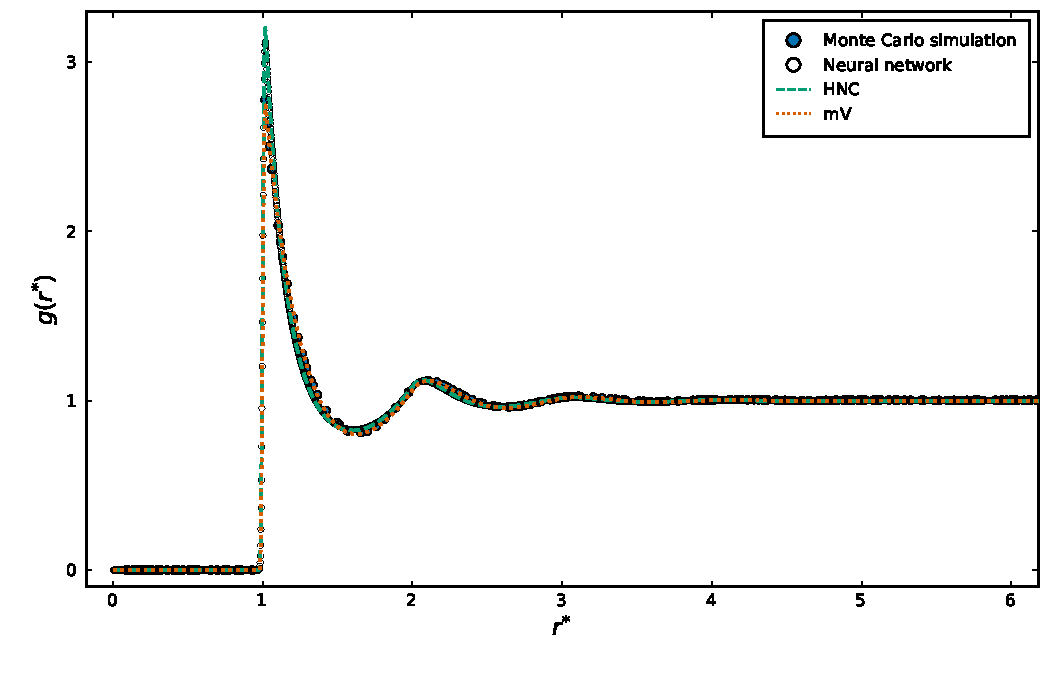
\includegraphics[width=\textwidth]{figuras/capitulo-3/comparison_p=0.35.pdf}
    \caption[Radial distribution function, $\phi=0.35$.]{The radial distribution function for density value $\phi=0.35$ obtained from computer simulations, and three different approximations:
    \begin{enumerate*}[label=(\alph*),itemjoin={,\enspace}]
        \item \emph{mV}, modified Verlet
        \item \emph{HNC}, Hypernetted Chain
        \item \emph{Neural network}, neural network approximation.
    \end{enumerate*}
    Inset shows the region close to the peak about $r^{*}=2$.
    }
    \label{fig:rdf35}
\end{figure}

\begin{figure}
    \centering
    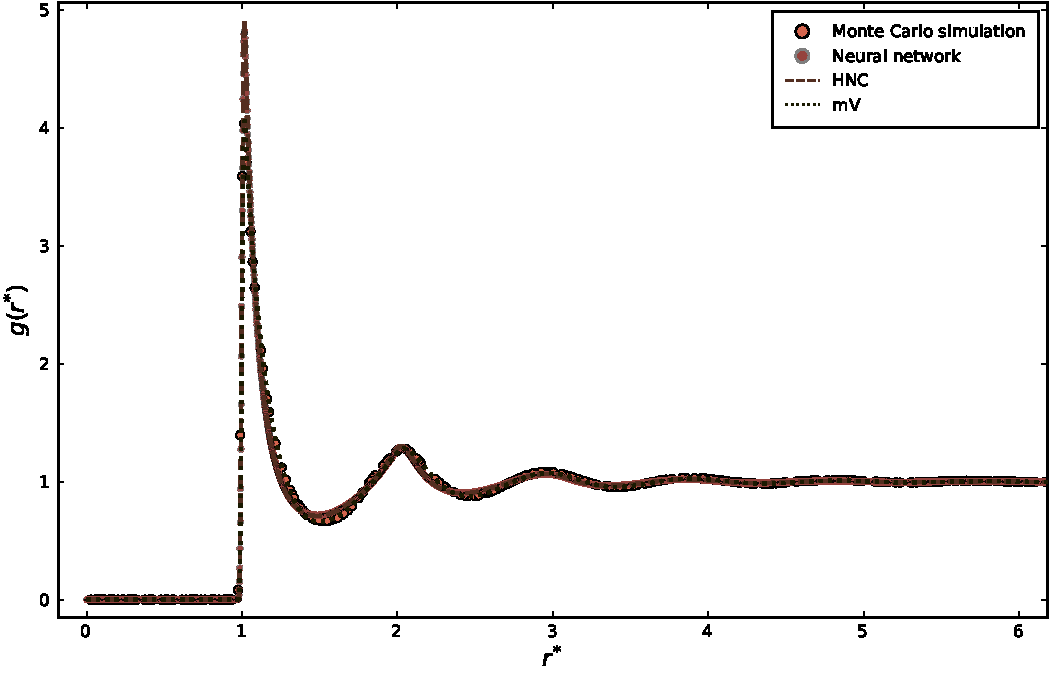
\includegraphics[width=\textwidth]{figuras/capitulo-3/comparison_p=0.45.pdf}
    \caption[Radial distribution function, $\phi=0.45$.]{The radial distribution function for density value $\phi=0.45$ obtained from computer simulations, and three different approximations:
    \begin{enumerate*}[label=(\alph*),itemjoin={,\enspace}]
        \item \emph{mV}, modified Verlet
        \item \emph{HNC}, Hypernetted Chain
        \item \emph{Neural network}, neural network approximation.
    \end{enumerate*}
    Inset shows the region close to the peak about $r^{*}=2$.
    }
    \label{fig:rdf45}
\end{figure}

\section{Discussion}
It would seem as though the neural network approximation reduces to the HNC
approximation, as seen in the results from the previous section. In this section
we shall investigate this matter in detail.
We will also continue the discussion of the results presented and try to make sense
of the training dynamics of the neural network. This is an important topic to
address due to the clear results that the neural network provides almost the same
result as the HNC approximation.

\subsection{Weight evolution of the neural network}

\begin{figure}
    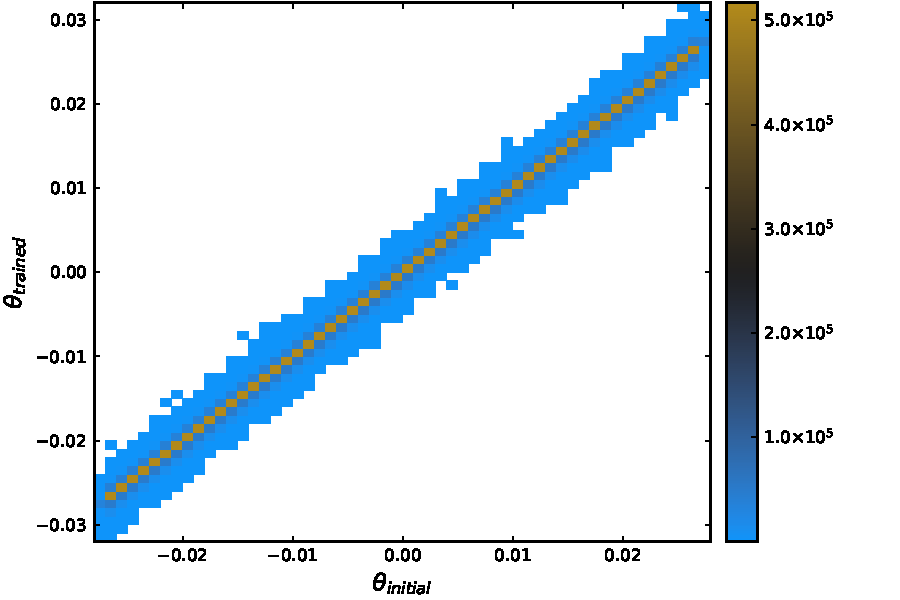
\includegraphics[width=\textwidth]{figuras/capitulo-3/weights_phi=0.15.pdf}
    \caption[Comparison between weights, $\phi=0.15$.]{Relation between the trained weights and the initial weights of $\nnet$ for the density value $\phi=0.15$. The scale on the right-hand side represents the total number of instances for the trained-initial pair of weights.} 
    \label{fig:pesos15}
\end{figure}

\begin{figure}
    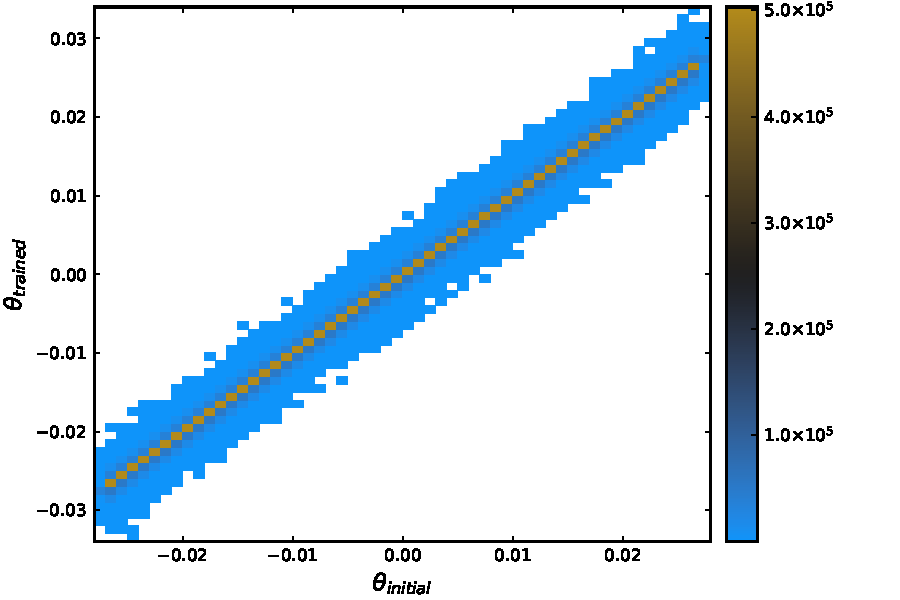
\includegraphics[width=\textwidth]{figuras/capitulo-3/weights_phi=0.25.pdf}
    \caption[Comparison between weights, $\phi=0.25$.]{Relation between the trained weights and the initial weights of $\nnet$ for the density value $\phi=0.25$. The scale on the right-hand side represents the total number of instances for the trained-initial pair of weights.}
    \label{fig:pesos25}
\end{figure}

\begin{figure}
    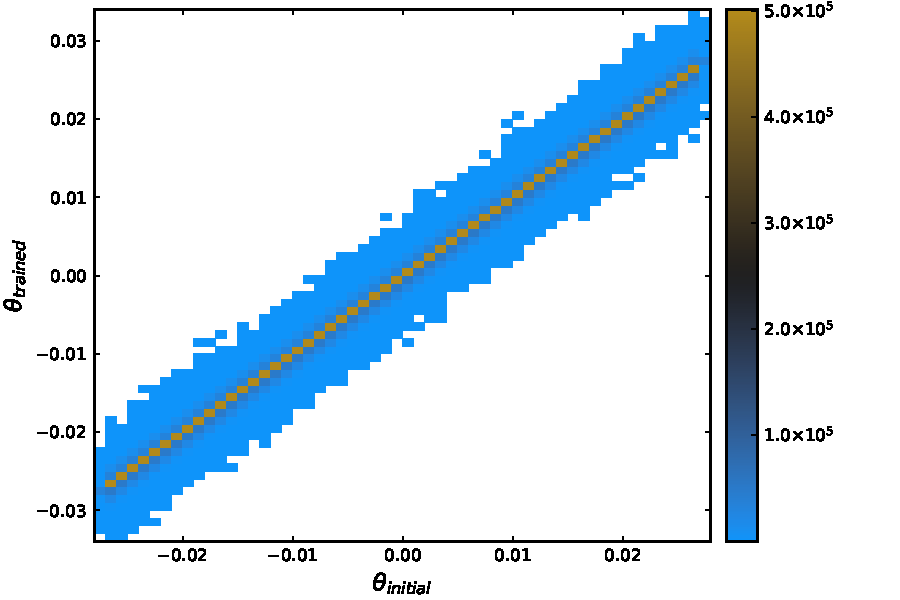
\includegraphics[width=\textwidth]{figuras/capitulo-3/weights_phi=0.35.pdf}
    \caption[Comparison between weights, $\phi=0.35$.]{Relation between the trained weights and the initial weights of $\nnet$ for the density value $\phi=0.35$. The scale on the right-hand side represents the total number of instances for the trained-initial pair of weights.}
    \label{fig:pesos35}
\end{figure}

\begin{figure}
    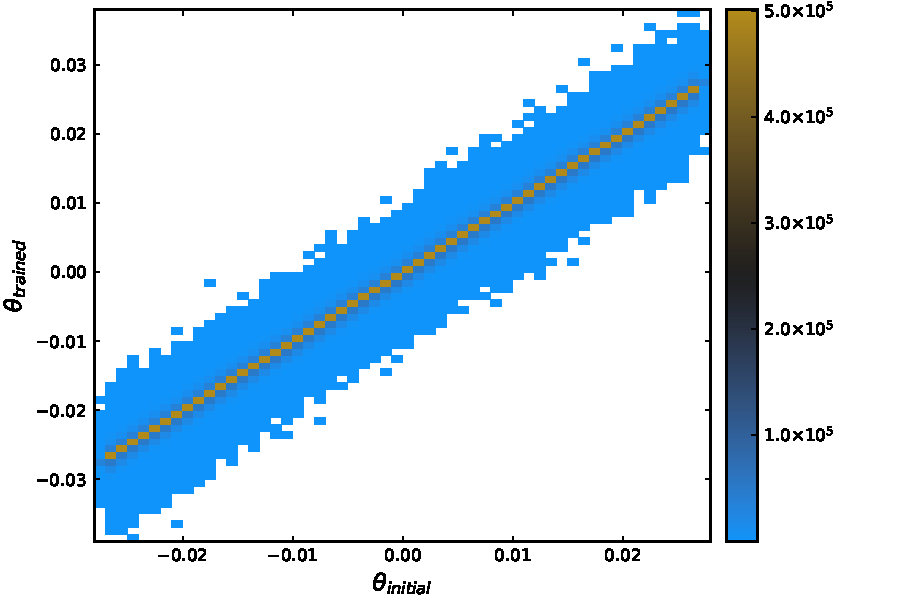
\includegraphics[width=\textwidth]{figuras/capitulo-3/weights_phi=0.45.pdf}
    \caption[Comparison between weights, $\phi=0.45$.]{Relation between the trained weights and the initial weights of $\nnet$ for the density value $\phi=0.45$. The scale on the right-hand side represents the total number of instances for the trained-initial pair of weights.}
    \label{fig:pesos45}
\end{figure}

We shall now examine the evolution of the weights $\theta$ from
$\nnet$, from the moment it was initialized to the moment its training finalized.
A histogram of this for each density value can be seen in
figures~(\ref{fig:pesos15}, \ref{fig:pesos25}, \ref{fig:pesos35}, \ref{fig:pesos45}).
We can observe that the way the weights show a diagonal represent a linear relationship 
between the initial weights, $\theta_{i}$, and the trained weights, $\theta_{t}$. In other 
words, the weights follow the linear expression
$\theta_{t} = \alpha \theta_{i} + \beta + \epsilon$, with
$\epsilon \sim \mathcal{N}(\mu, \sigma^{2})$ a normal random variable with mean
$\mu$ and variance $\sigma^2$. The noise term can be any other continuous probability 
distribution, but without loss of generality the normal distribution was chosen for
our purposes. For now, we are not interested in the values of $\alpha$ or $\beta$,
but merely on the linear relationship between them.

One thing to notice is the fact that the higher the value for the density, the larger
the variance is. If we observe the variance for the density $\phi=0.15$ in figure~\ref{fig:pesos15}
we see that the variance is small due to the fact that the blue shaded region around
the diagonal is close to it. If we now see the same figure~\ref{fig:pesos45} for the 
density value of $\phi=0.45$ we see that this shaded region is significantly larger.
This would mean that, at higher densities, the weights of $\nnet$ are more spread out
from the mean, and the neural network might have adjusted its weights to account for
different computations of the bridge function.

The most interesting part of this is the fact that the weights from initialization
do not change much throughout the training scheme, which would imply that a local minimum
has already been found. This might be the case, for the HNC is actually a solution to
the OZ equation, and solutions around this particular approximation might be as well 
solutions. This, however, does not answer the question of why the spread is larger when
higher densities are inspected.

\subsection{The Hypernetted Chain approximation as a stable minimum}
It would seem that the way the weights are updated, albeit with minimal change from its
initial values, is due to the fact of having reached a minimum already.
We must recall that the weight update and neural network training is essentially an
optimization problem~\eqref{eq:optimizacion}, and the main goal is to find a minimum
of the cost function~\eqref{eq:costo}. With the results presented so far, it might be
possible to postulate that the \emph{HNC approximation is a stable minimum} for the
neural network $\nnet$.
This would answer the question of why the weights of the neural network during training
explored in the previous section did not change very much throughout the numerical scheme.
Because if we have already found a minimum, the optimization algorithm might end up
oscillating in the proximity of this value.

On the other hand, this idea could also give answer to the question of why the spread
is large for higher density values. If we pay close attention to the approximation
results for the \emph{low density} values in figure~\ref{fig:rdf15}, we can see that
although every approximation given a low accuracy estimation of the second peak as shown
in the inset, for the main peak, the neural network approximation is very accurate.
If we now observe the figure~\ref{fig:rdf45} which refers to the \emph{high density} value
we can see that the estimation is quite poor.
Let us now relate this to the weight evolution. For the \emph{low density} regime, the 
weight evolution has a \emph{lower variance}; for the \emph{high density} regime, there
is now a \emph{higher variance} in the weight evolution.
This suggests that, for \emph{lower density} values, there was no need to adjust the
weights more than shown in figure~\ref{fig:pesos15} because the approximation is accurate
enough. However, for the \emph{higher density} values, the approximation is not good enough
and the optimization method was trying to adjust the weights accordingly, even if
unsuccessfully.

\subsection{Does the neural network reduce to HNC?}
For the low density regimes, HNC is an accurate approximation for the interaction potential.
Hence, the neural network is an accurate approximation. On the contrary, for high density
regimes, both approximation fail to provide an accurate solution.

If, in fact, the neural network is oscillating about zero (the HNC approximation), then
it makes sense that both estimations give the results observed. Yet, we cannot gaurantee
by any means possible that the neural network reduces to the HNC approximation.
We only possess \emph{statistical evidence} from the training dynamics that the neural
network weights do not change much throughout its training.

This observation might shed the light into possibilities of changing the way the neural
network propagates its values and return an output.

% TODO: Hablar sobre la poca desviación de los resultados, sobre todo hacer hincapié en el hecho de que, el no moverse mucho del cero implica que HNC es un mínimo estable y por lo tanto los pesos prefieren quedarse oscilando en este valor. Por otro lado, hablar sobre la importancia de que un valor aleatorio (o función aleatoria, matrices aleatorias, algo semejante) puede aproximar una función puente, pues esto no es algo trivial. Esto significa que se pueden aproximar las expansiones diagramáticas mediante procesos aleatorios, lo cual tiene implicaciones teóricas interesantes.
% TODO: El hecho de que los valores estén alejados del centro significa que la desviación de la media es grande. Esto puede implicar que, entre más cerca se esté del centro, menor es el cambio entre pesos entrenados e iniciales. Esto no da un argumento de porqué se reduce a HNC, sino que puede dar un argumento sobre la dinámica de entrenamiento. Esto puede ser el argumento de que quizás el hecho de que se queda alrededor de HNC porque es un mínimo ocasiona que los pesos no cambien demasiado al ser entrenados.
%\include{Chapters/Chapter2} 
%\include{Chapters/Chapter3}
%\include{Chapters/Chapter4} 
%\include{Chapters/Chapter5} 

%----------------------------------------------------------------------------------------
%	THESIS CONTENT - APPENDICES
%----------------------------------------------------------------------------------------

\appendix % Cue to tell LaTeX that the following "chapters" are Appendices

% Include the appendices of the thesis as separate files from the Appendices folder
% Uncomment the lines as you write the Appendices

% \include{Appendices/AppendixA}
%\include{Appendices/AppendixB}
%\include{Appendices/AppendixC}

%----------------------------------------------------------------------------------------
%	BIBLIOGRAPHY
%----------------------------------------------------------------------------------------

\printbibliography[heading=bibintoc]

%----------------------------------------------------------------------------------------

\end{document}  
